\section{Auswertung}

\subsection{Sphärische Aberration}

\subsection{Koma}

\begin{figure}[htb]
	\begin{minipage}[t]{0.32\textwidth}
		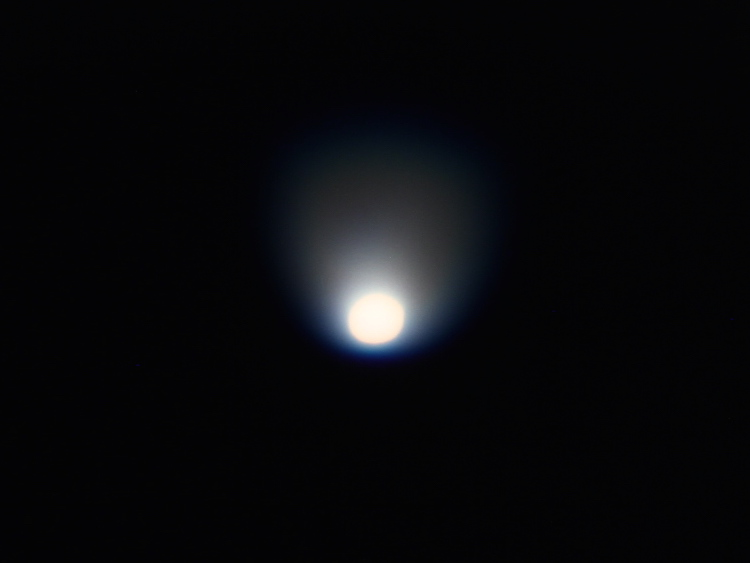
\includegraphics[width=\linewidth]{img/Koma/Prakt_Linsenfehler_2015_06_04_097}
		\label{fig:koma_stark}
		\caption{Starkes Koma am Außenrand der Linse}
	\end{minipage}
	\hfill
	\begin{minipage}[t]{0.32\textwidth}
		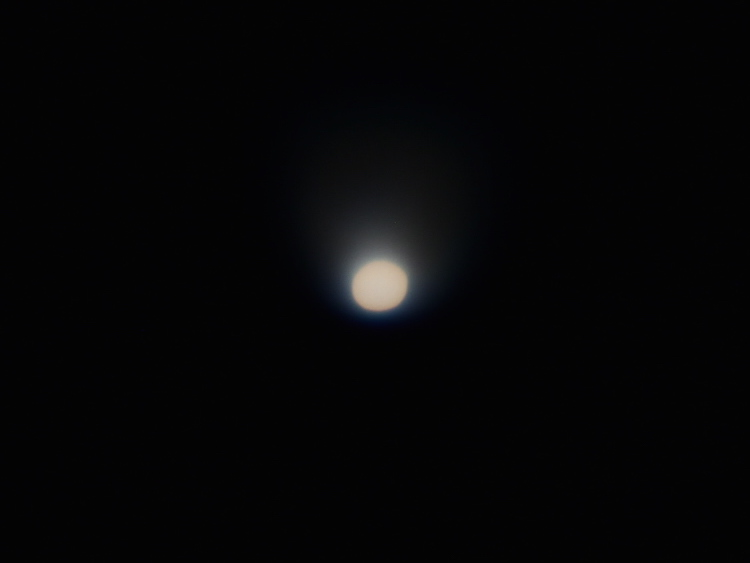
\includegraphics[width=\linewidth]{img/Koma/Prakt_Linsenfehler_2015_06_04_096}
		\label{fig:koma_schwach}
		\caption{Schwaches Koma nahe der optischen Achse}
	\end{minipage}
	\hfill
	\begin{minipage}[t]{0.32\textwidth}
		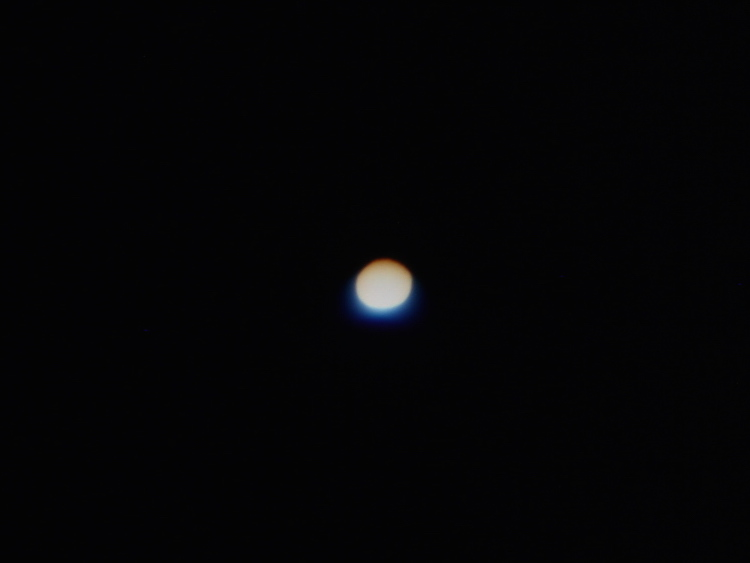
\includegraphics[width=\linewidth]{img/Koma/Prakt_Linsenfehler_2015_06_04_099}
		\label{fig:koma_korrigiert}
		\caption{Abbildung mit Korrektur der Koma}
	\end{minipage}	
\end{figure}

\subsection{Astigmatismus}

\begin{figure}[htb]
	\begin{minipage}[t]{0.48\textwidth}
		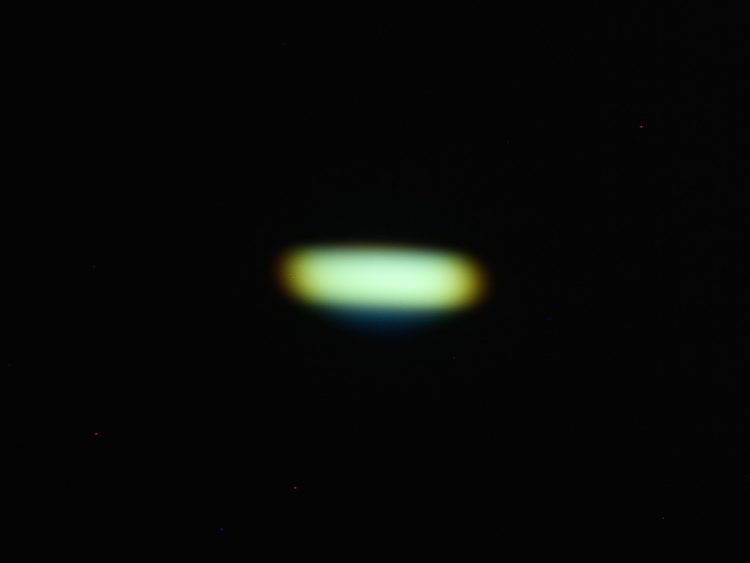
\includegraphics[width=\linewidth]{img/Astigmatismus/Prakt_Linsenfehler_2015_06_04_087_saggital}
		\label{fig:astigmatismus_saggital}
		\caption{Abbildung der Saggitalebene}
	\end{minipage}
	\hfill
	\begin{minipage}[t]{0.48\textwidth}
		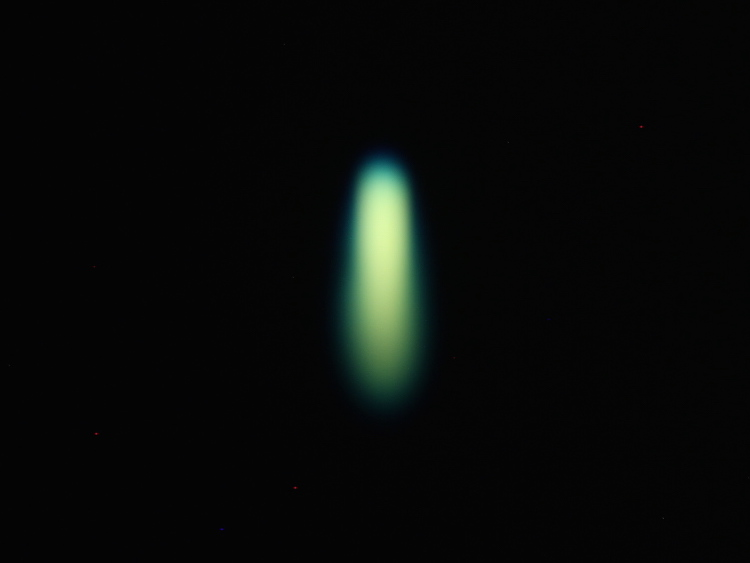
\includegraphics[width=\linewidth]{img/Astigmatismus/Prakt_Linsenfehler_2015_06_04_088_meridional}
		\label{fig:astigmatismus_meridional}
		\caption{Abbildung der Meridionalebene}
	\end{minipage}
	
	\vspace{0.5cm}
	
	\begin{minipage}[t]{0.48\textwidth}
		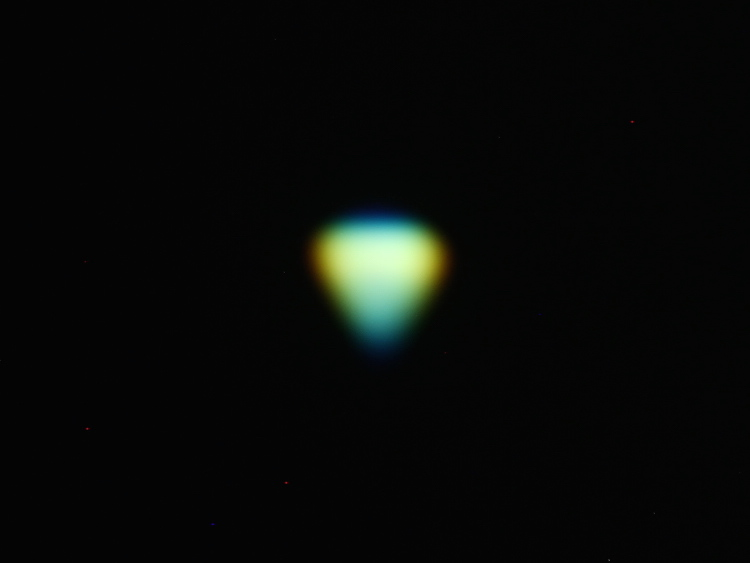
\includegraphics[width=\linewidth]{img/Astigmatismus/Prakt_Linsenfehler_2015_06_04_089_mittenfokus}
		\label{fig:astigmatismus_mittenfokus}
		\caption{Fokus zwischen meridionaler und saggitaler Abbildung}
	\end{minipage}
	\hfill
	\begin{minipage}[t]{0.48\textwidth}
		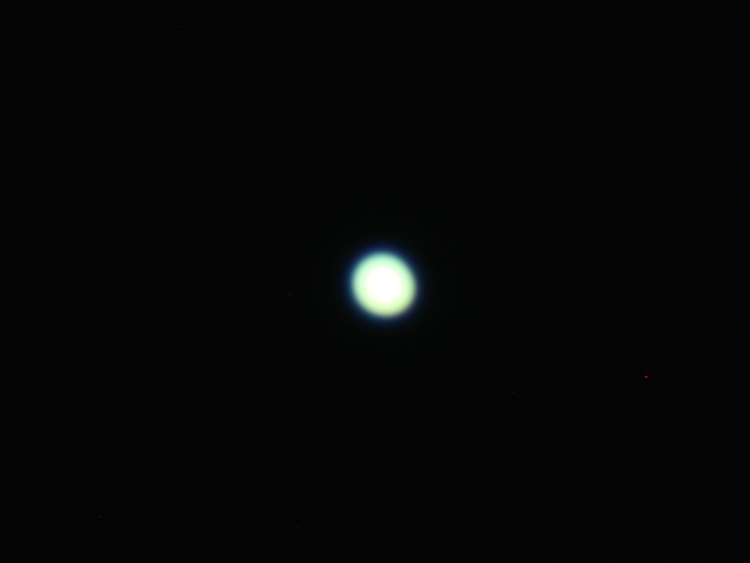
\includegraphics[width=\linewidth]{img/Astigmatismus/Prakt_Linsenfehler_2015_06_04_086}
		\label{fig:astigmatismus_korrigiert}
		\caption{Korrektur des Astigmatismus}
	\end{minipage}
\end{figure}

\subsection{Bildfeldwölbung}

\begin{figure}[htb]
	\begin{minipage}[t]{0.48\textwidth}
		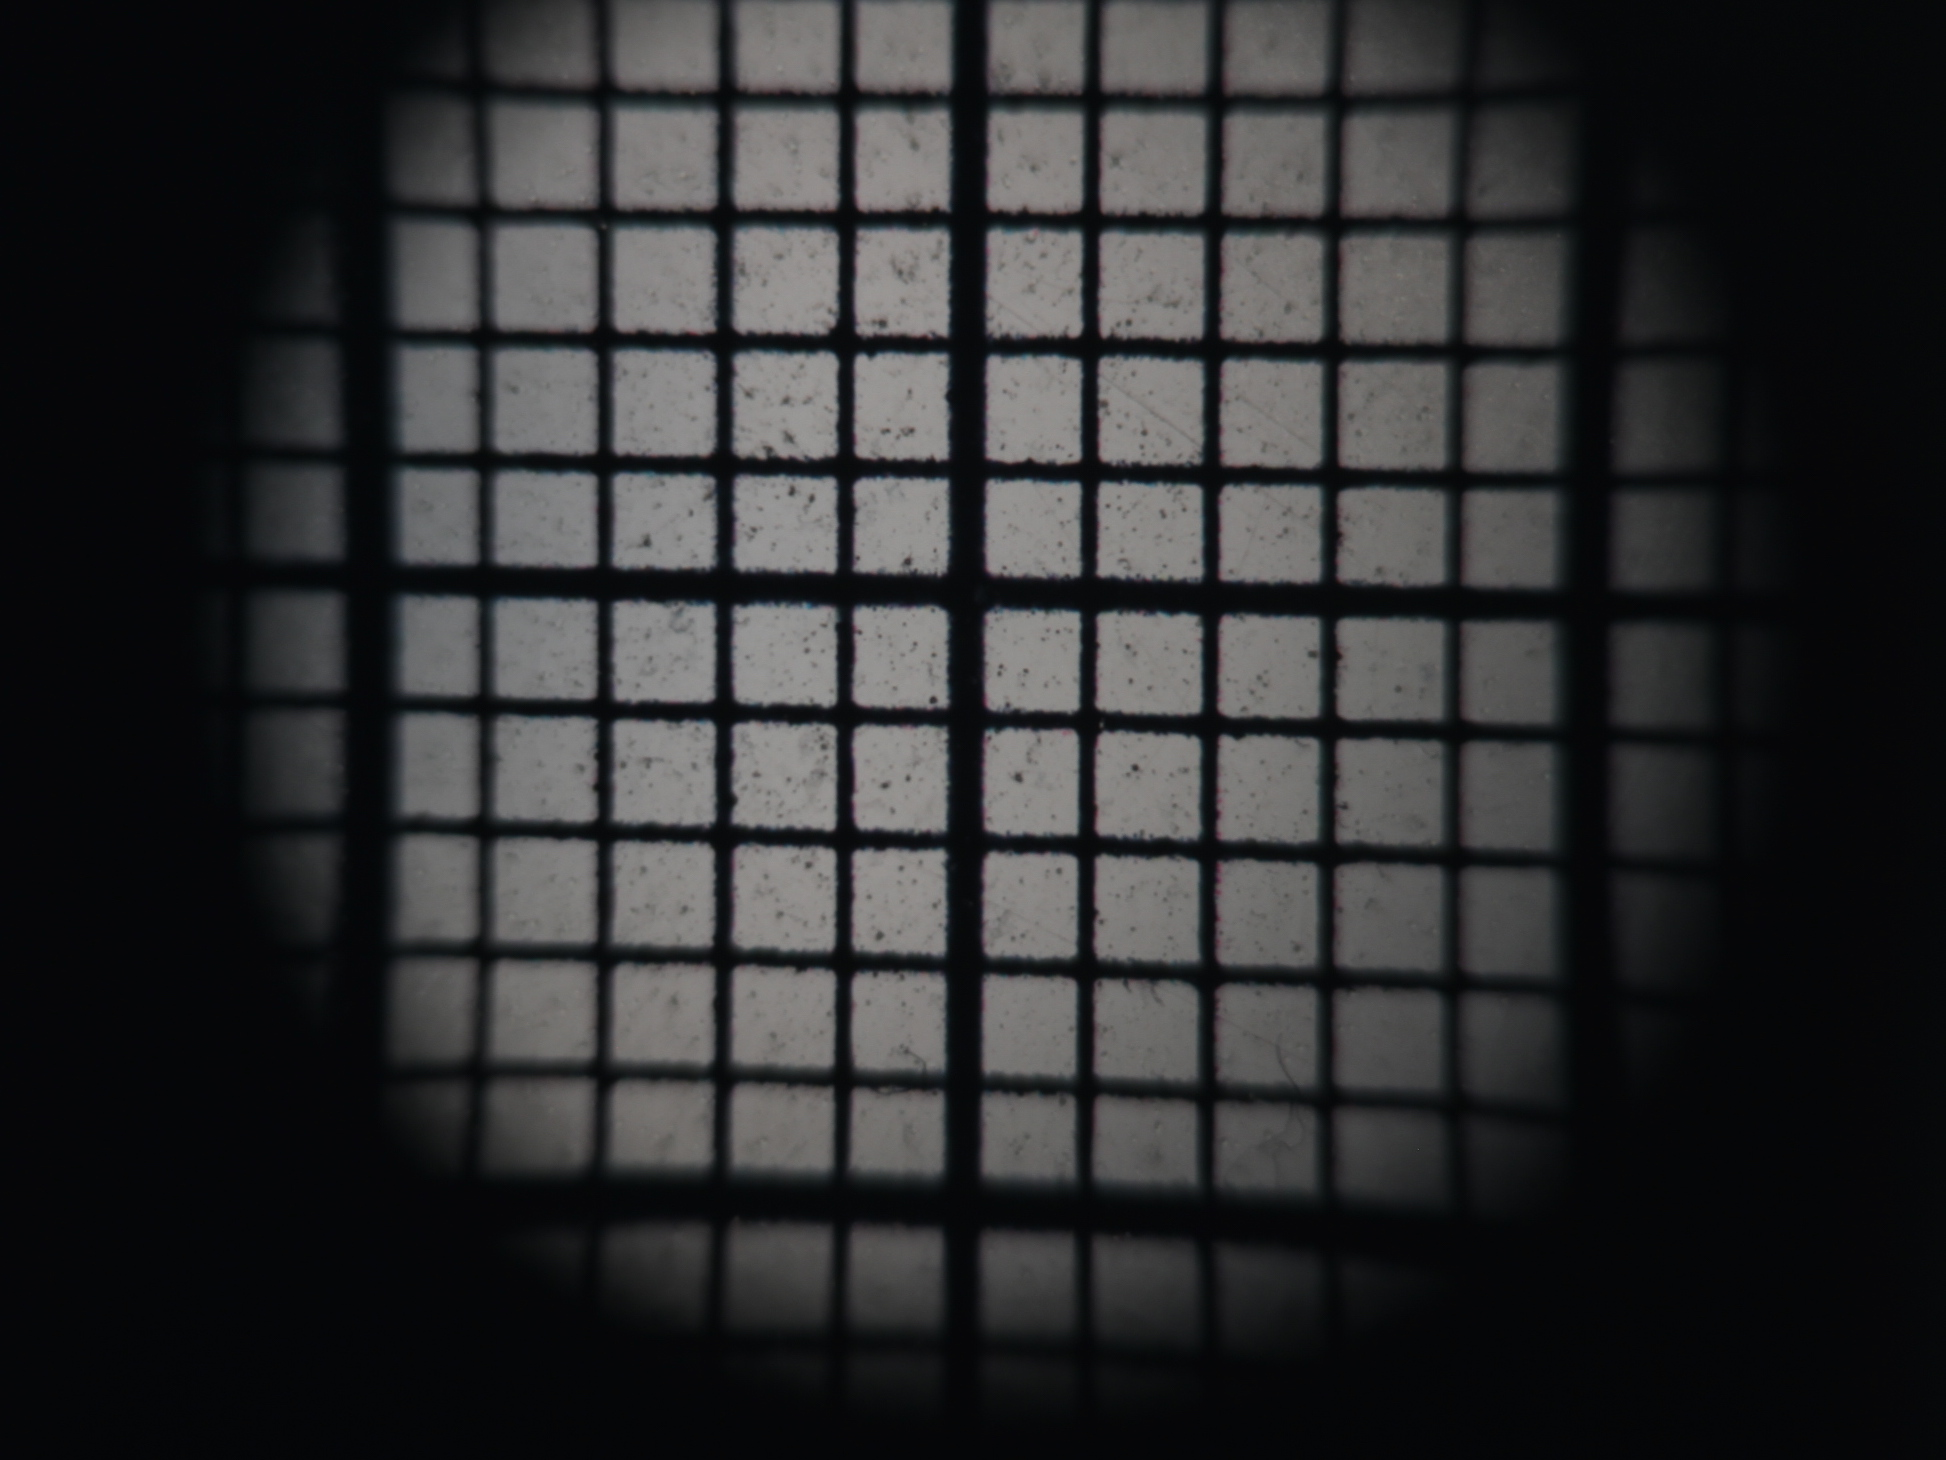
\includegraphics[width=\linewidth]{img/Bildwoelbung/Prakt_Linsenfehler_2015_06_04_074}
		\label{fig:bildwoelbung_aussen}
		\caption{Unschärfe am Außenrand des Gitters}
	\end{minipage}
	\hfill
	\begin{minipage}[t]{0.48\textwidth}
		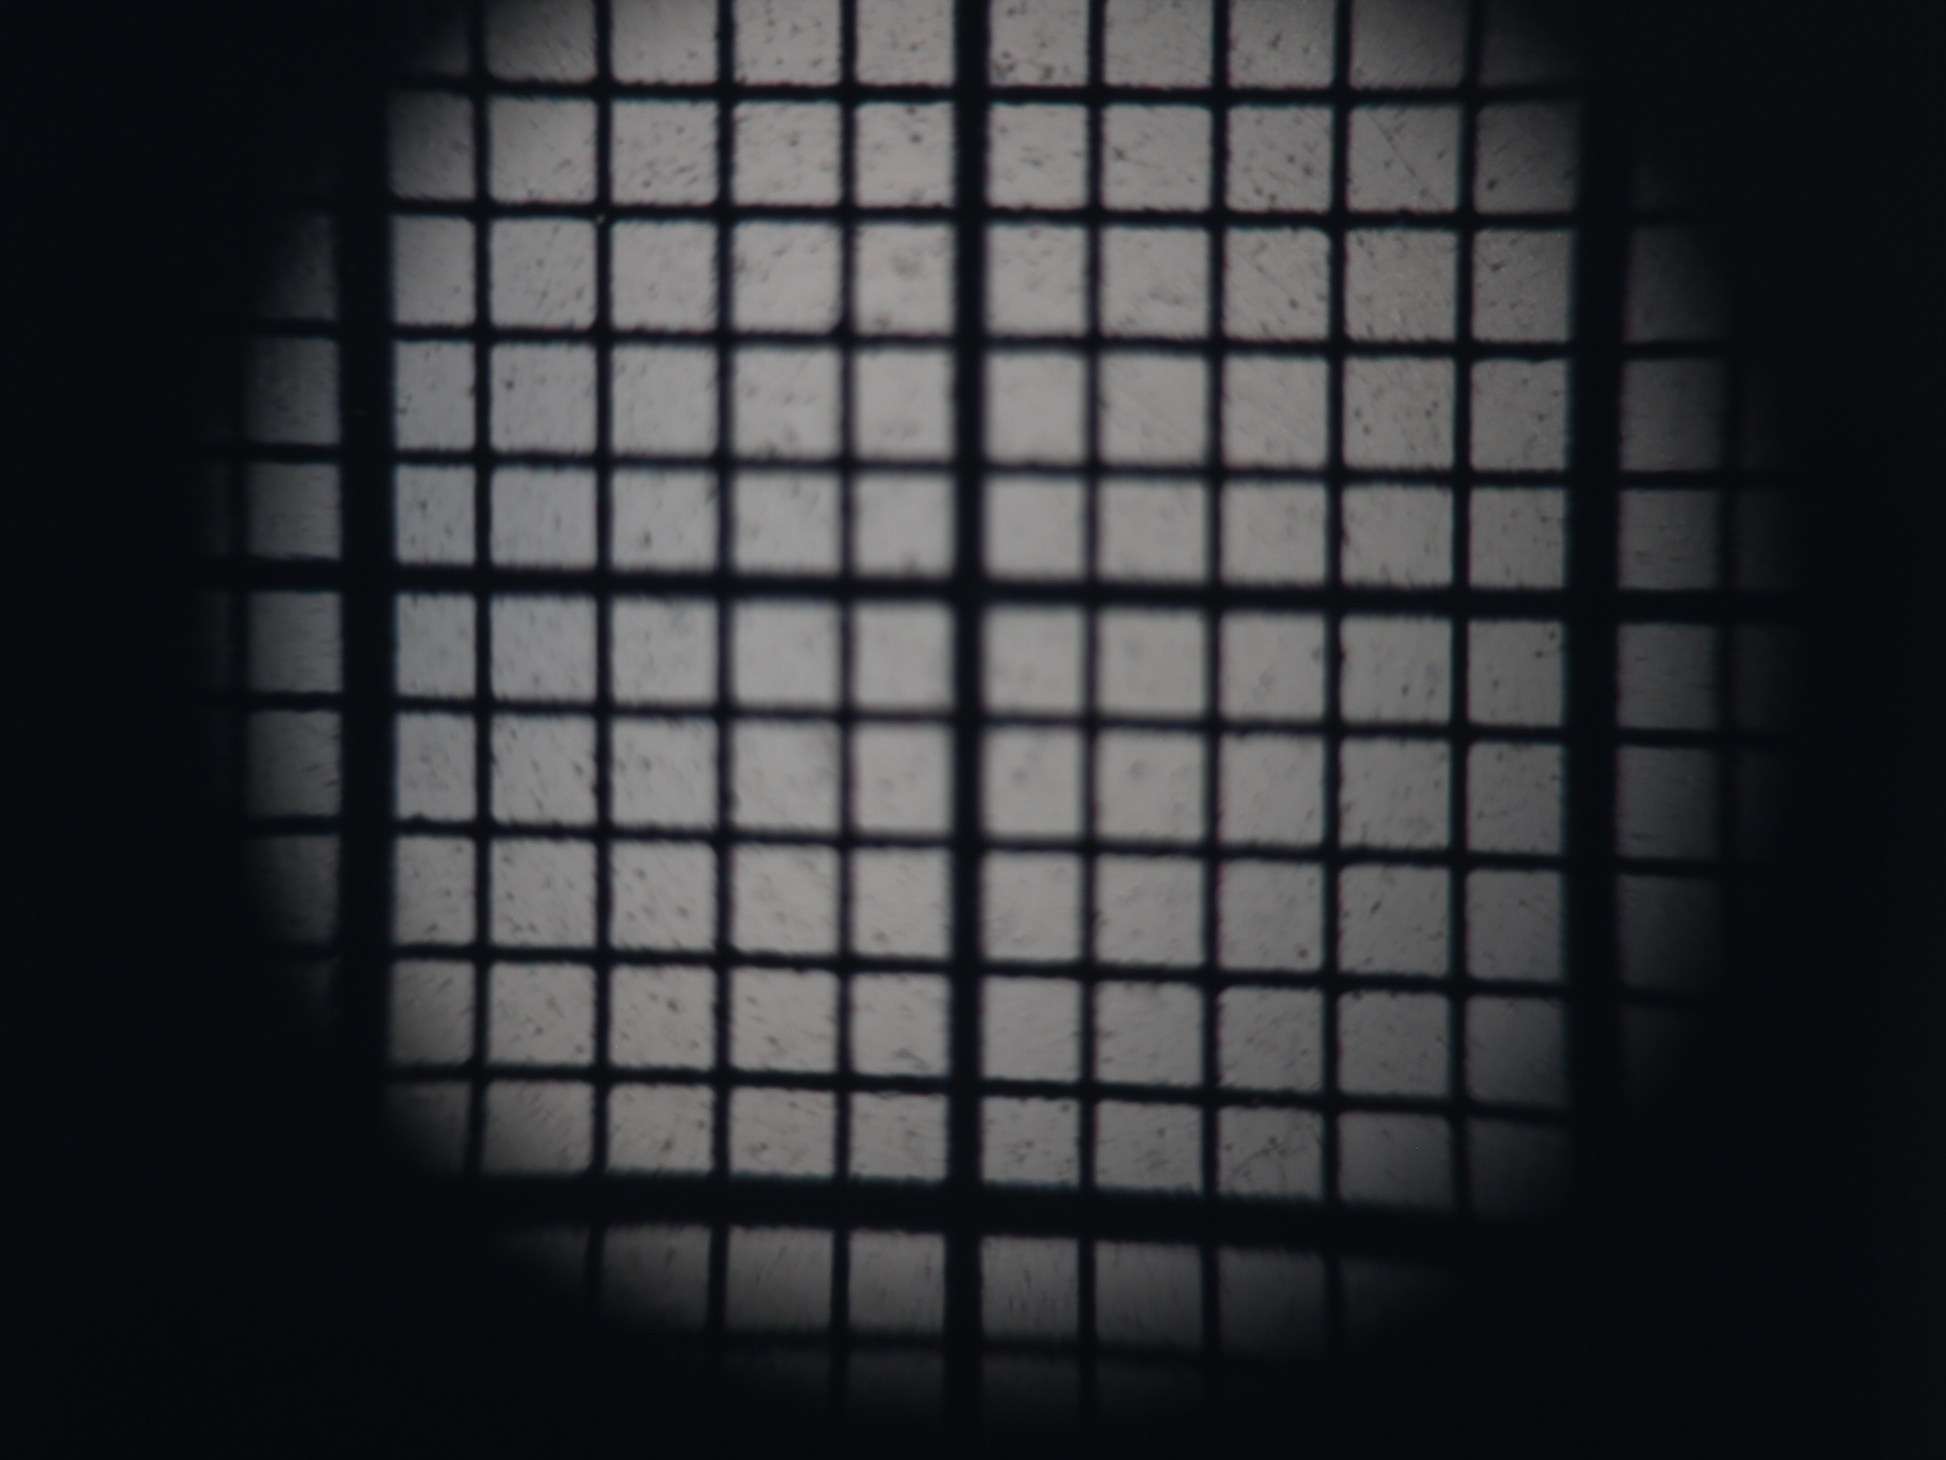
\includegraphics[width=\linewidth]{img/Bildwoelbung/Prakt_Linsenfehler_2015_06_04_075}
		\label{fig:bildwoelbung_korrigiert}
		\caption{Unschärfe in der Mitte des Gitters}
	\end{minipage}
\end{figure}

\begin{figure}[htb]
	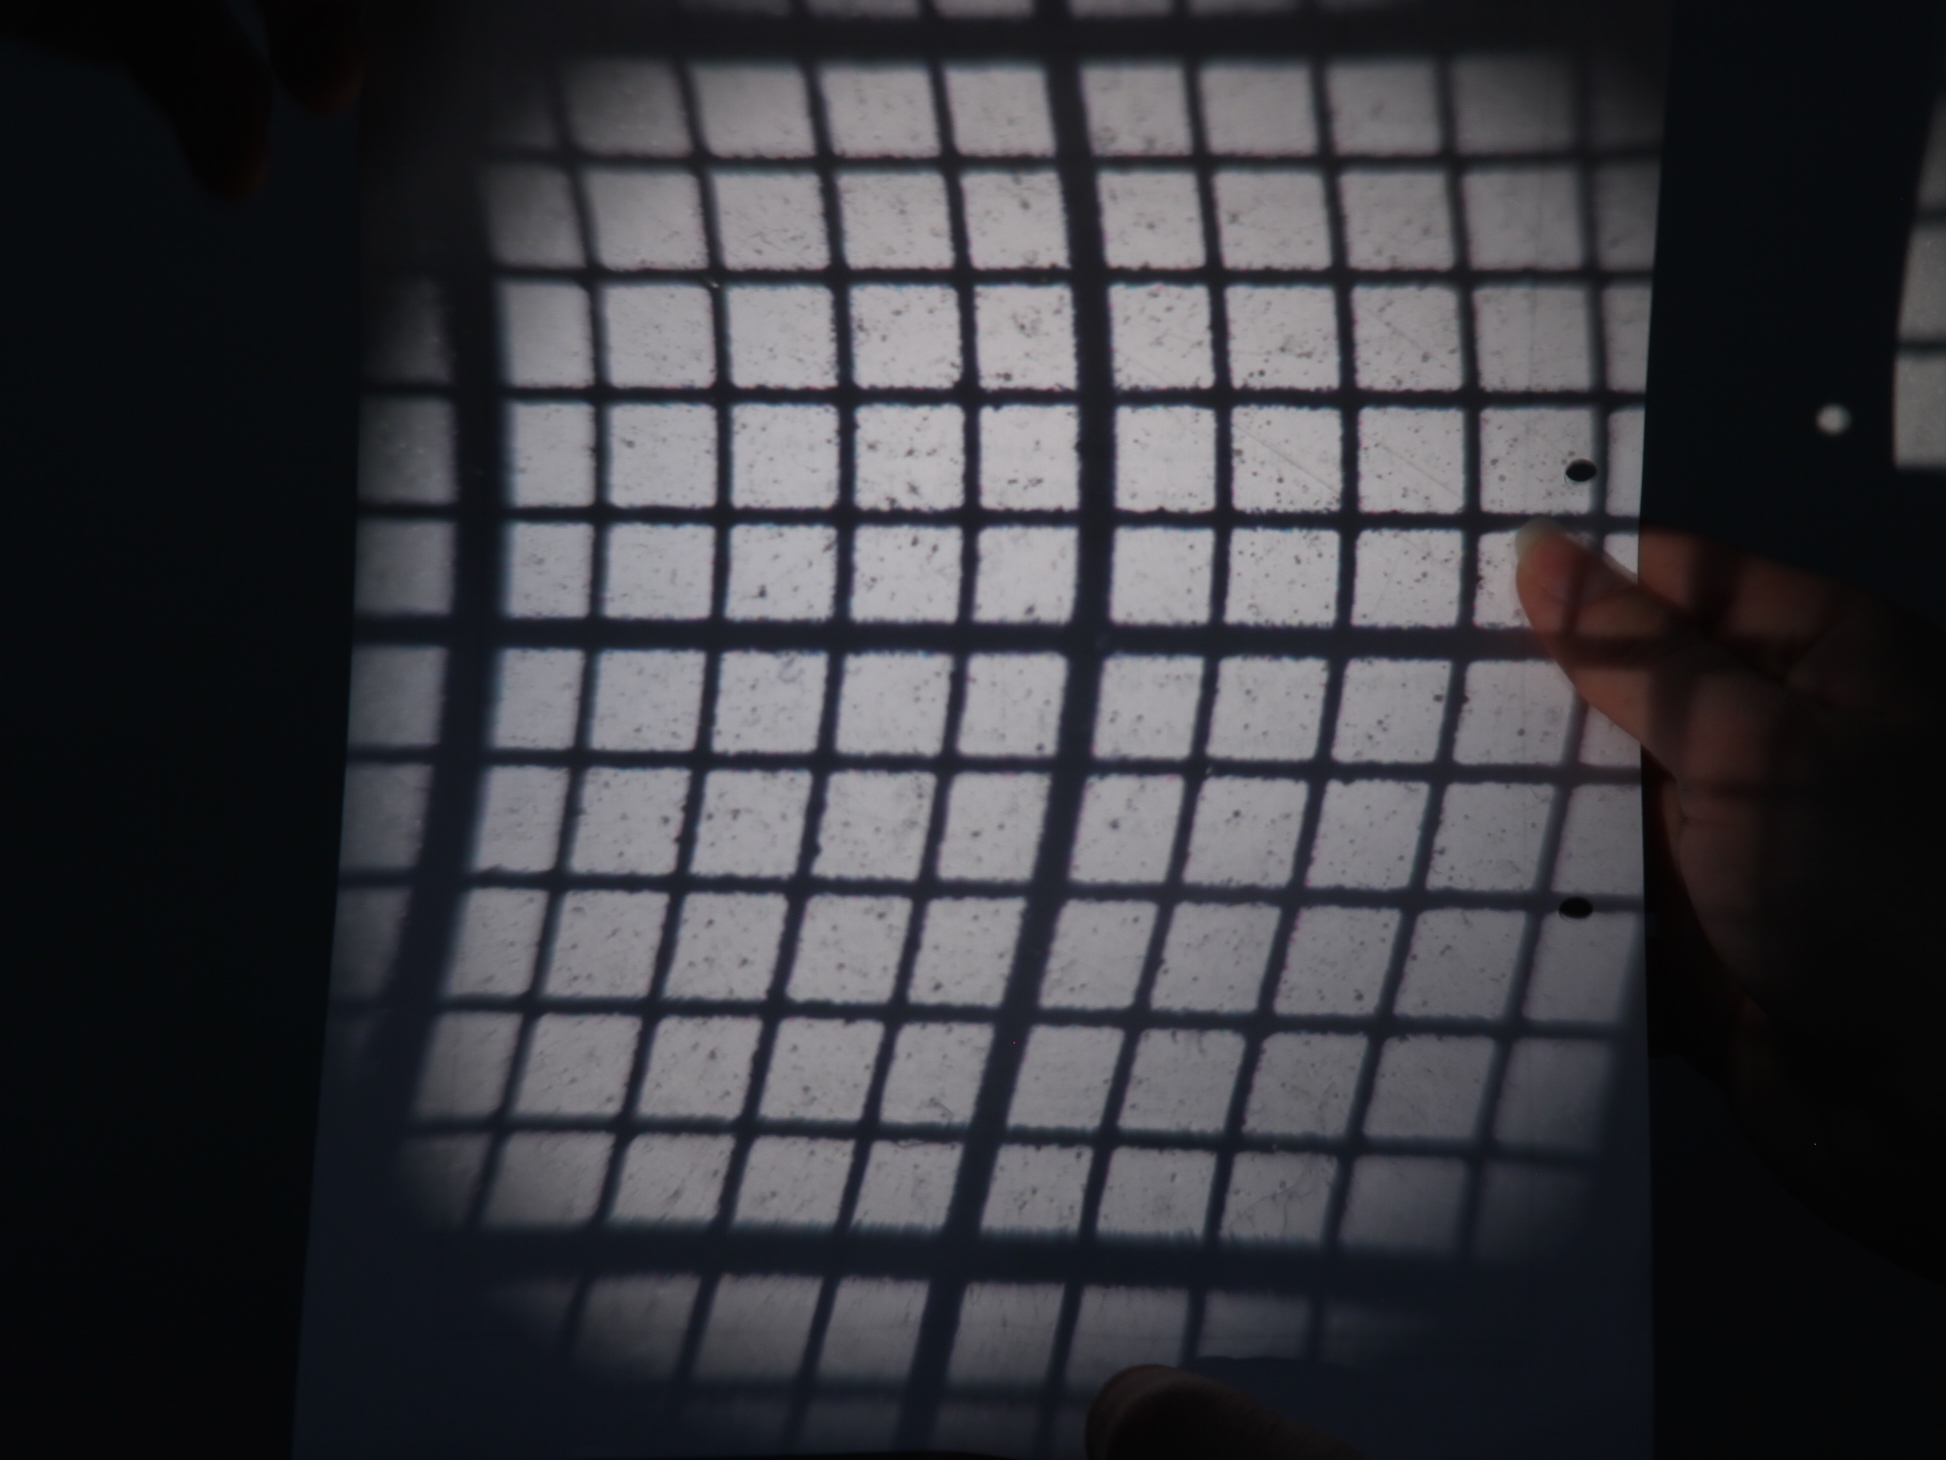
\includegraphics[width=\linewidth]{img/Bildwoelbung/Prakt_Linsenfehler_2015_06_04_076}
	\label{fig:bildwoelbung_korrigiert}
	\caption{Korrektur der Bildfeldwölbung durch gekrümmten Projektionsschirm}
\end{figure}

\subsection{Verzeichnung}

\begin{figure}[htb]
	\begin{minipage}[t]{0.48\textwidth}
		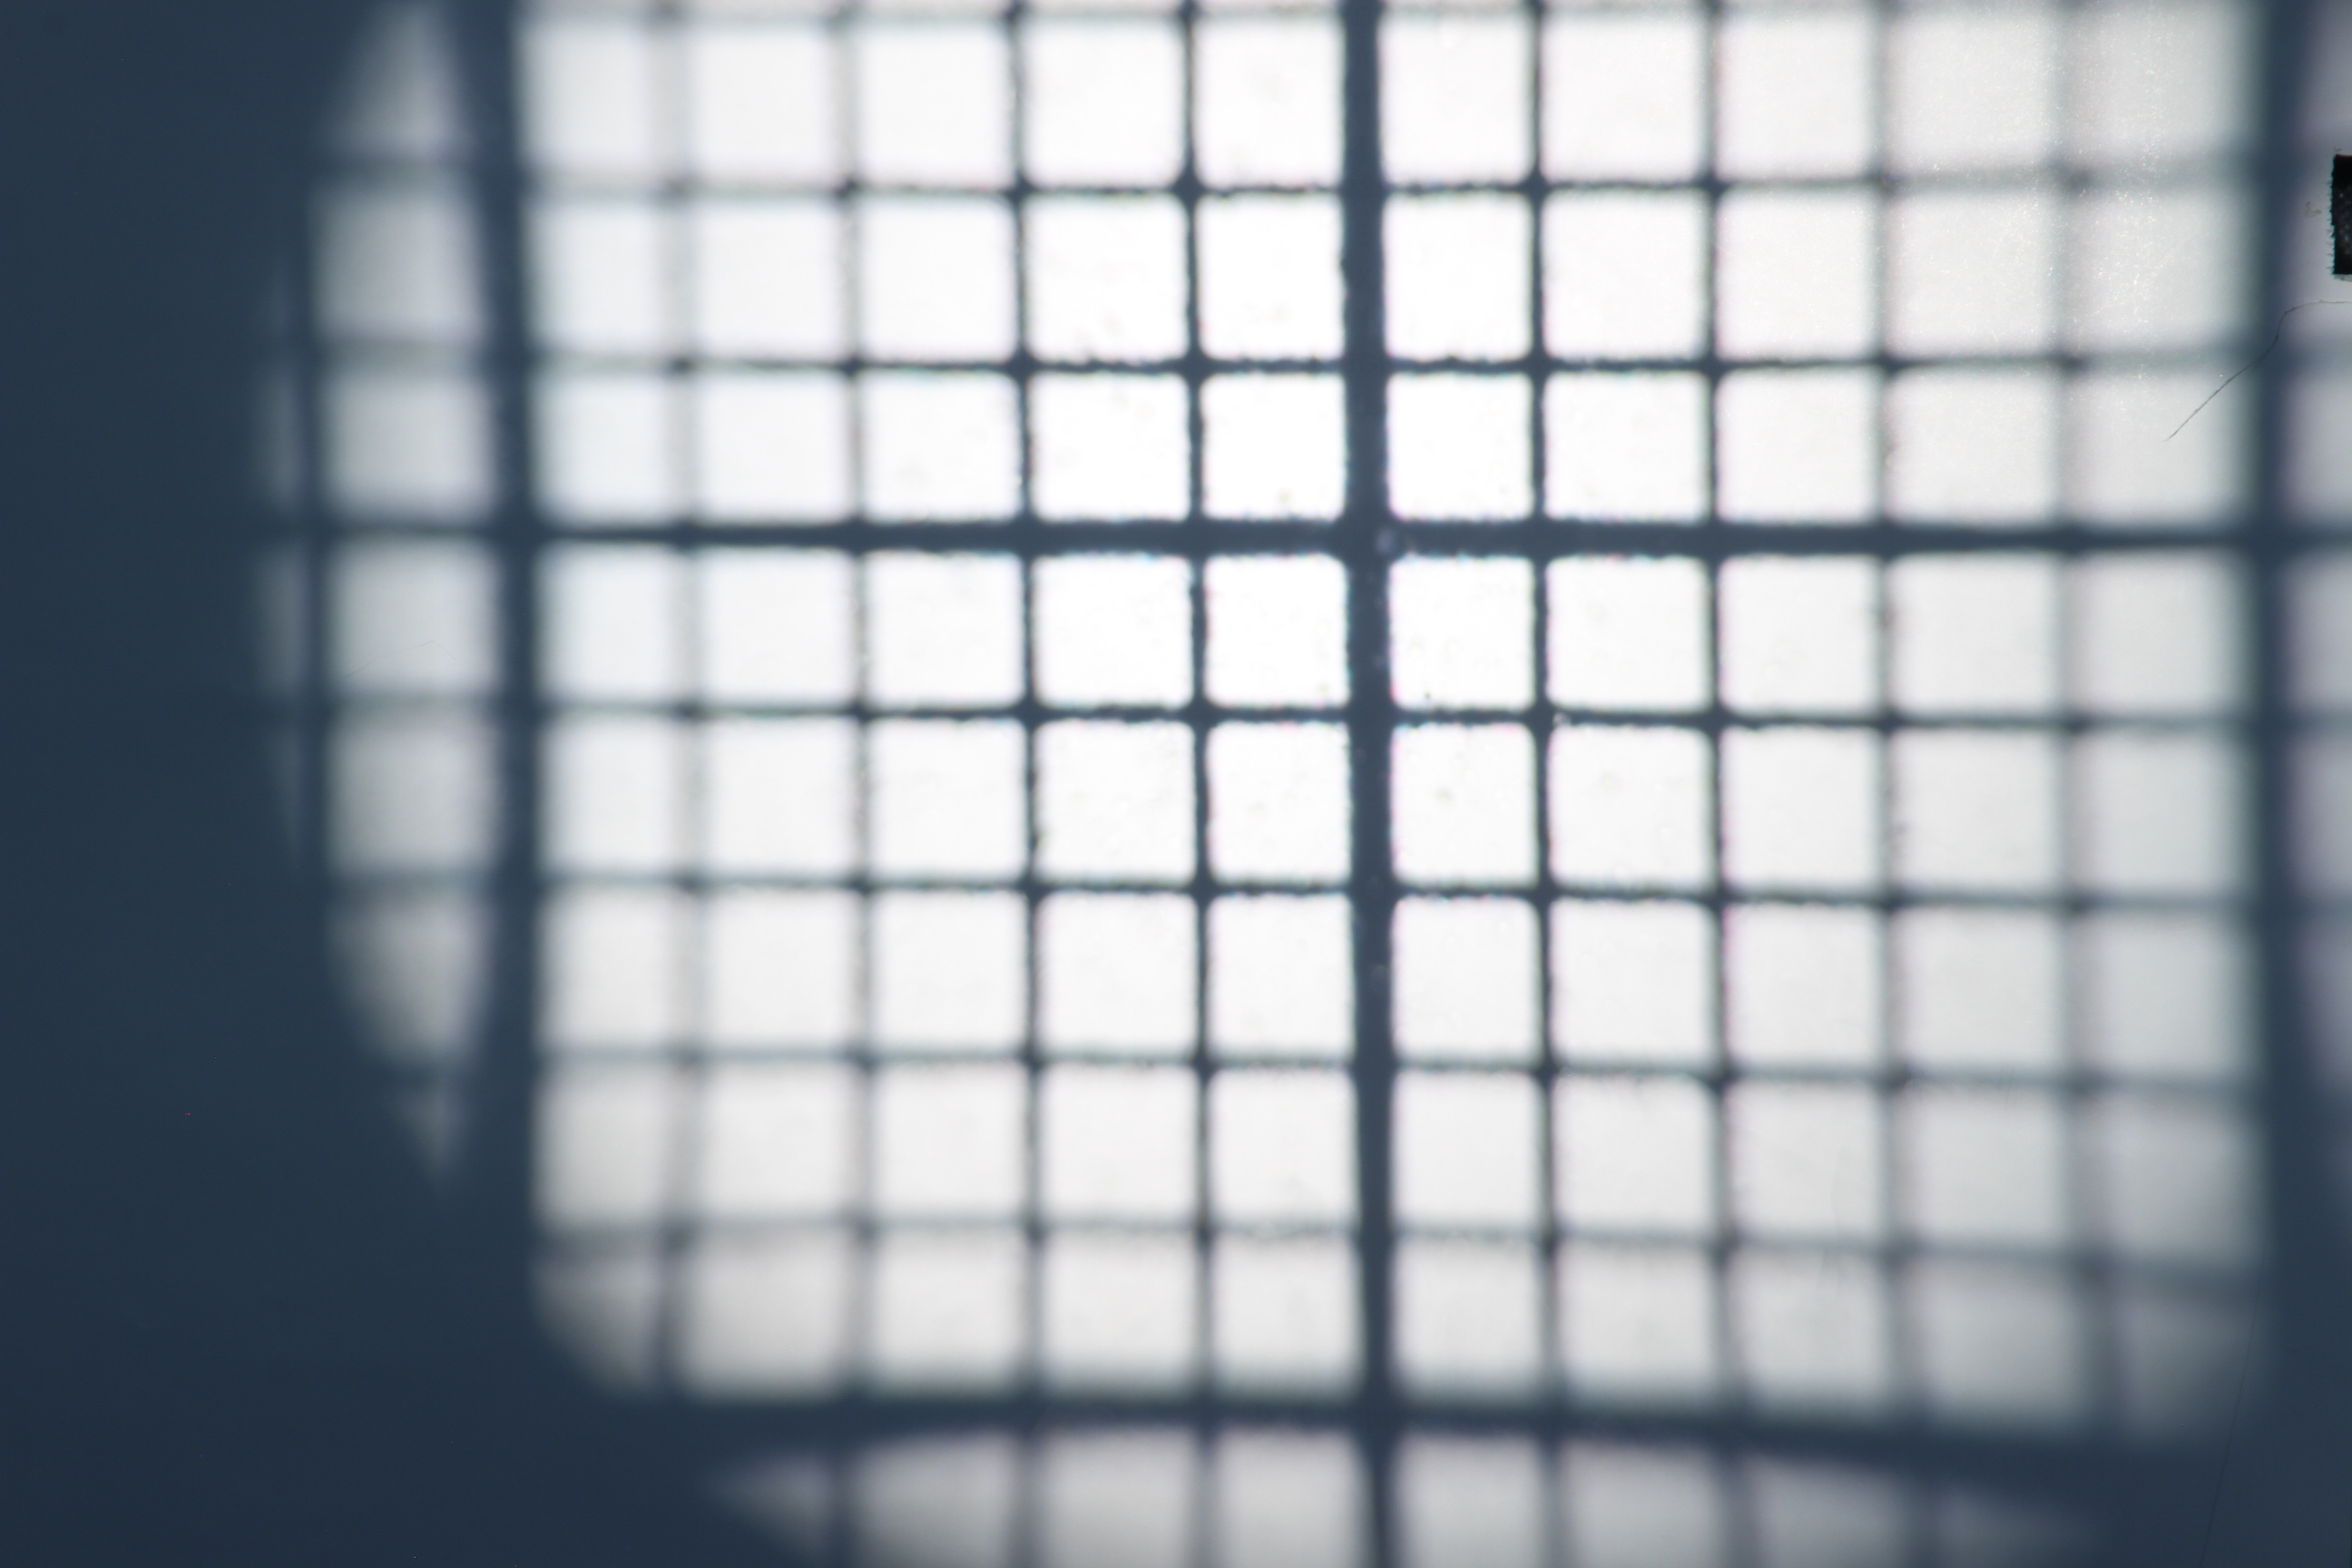
\includegraphics[width=\linewidth]{img/Verzeichnung/Prakt_Linsenfehler_2015_06_04_082}
		\label{fig:verzeichnung}
		\caption{Am Rand des Gitters erkennbare Krümmung}
	\end{minipage}
	\hfill
	\begin{minipage}[t]{0.48\textwidth}
		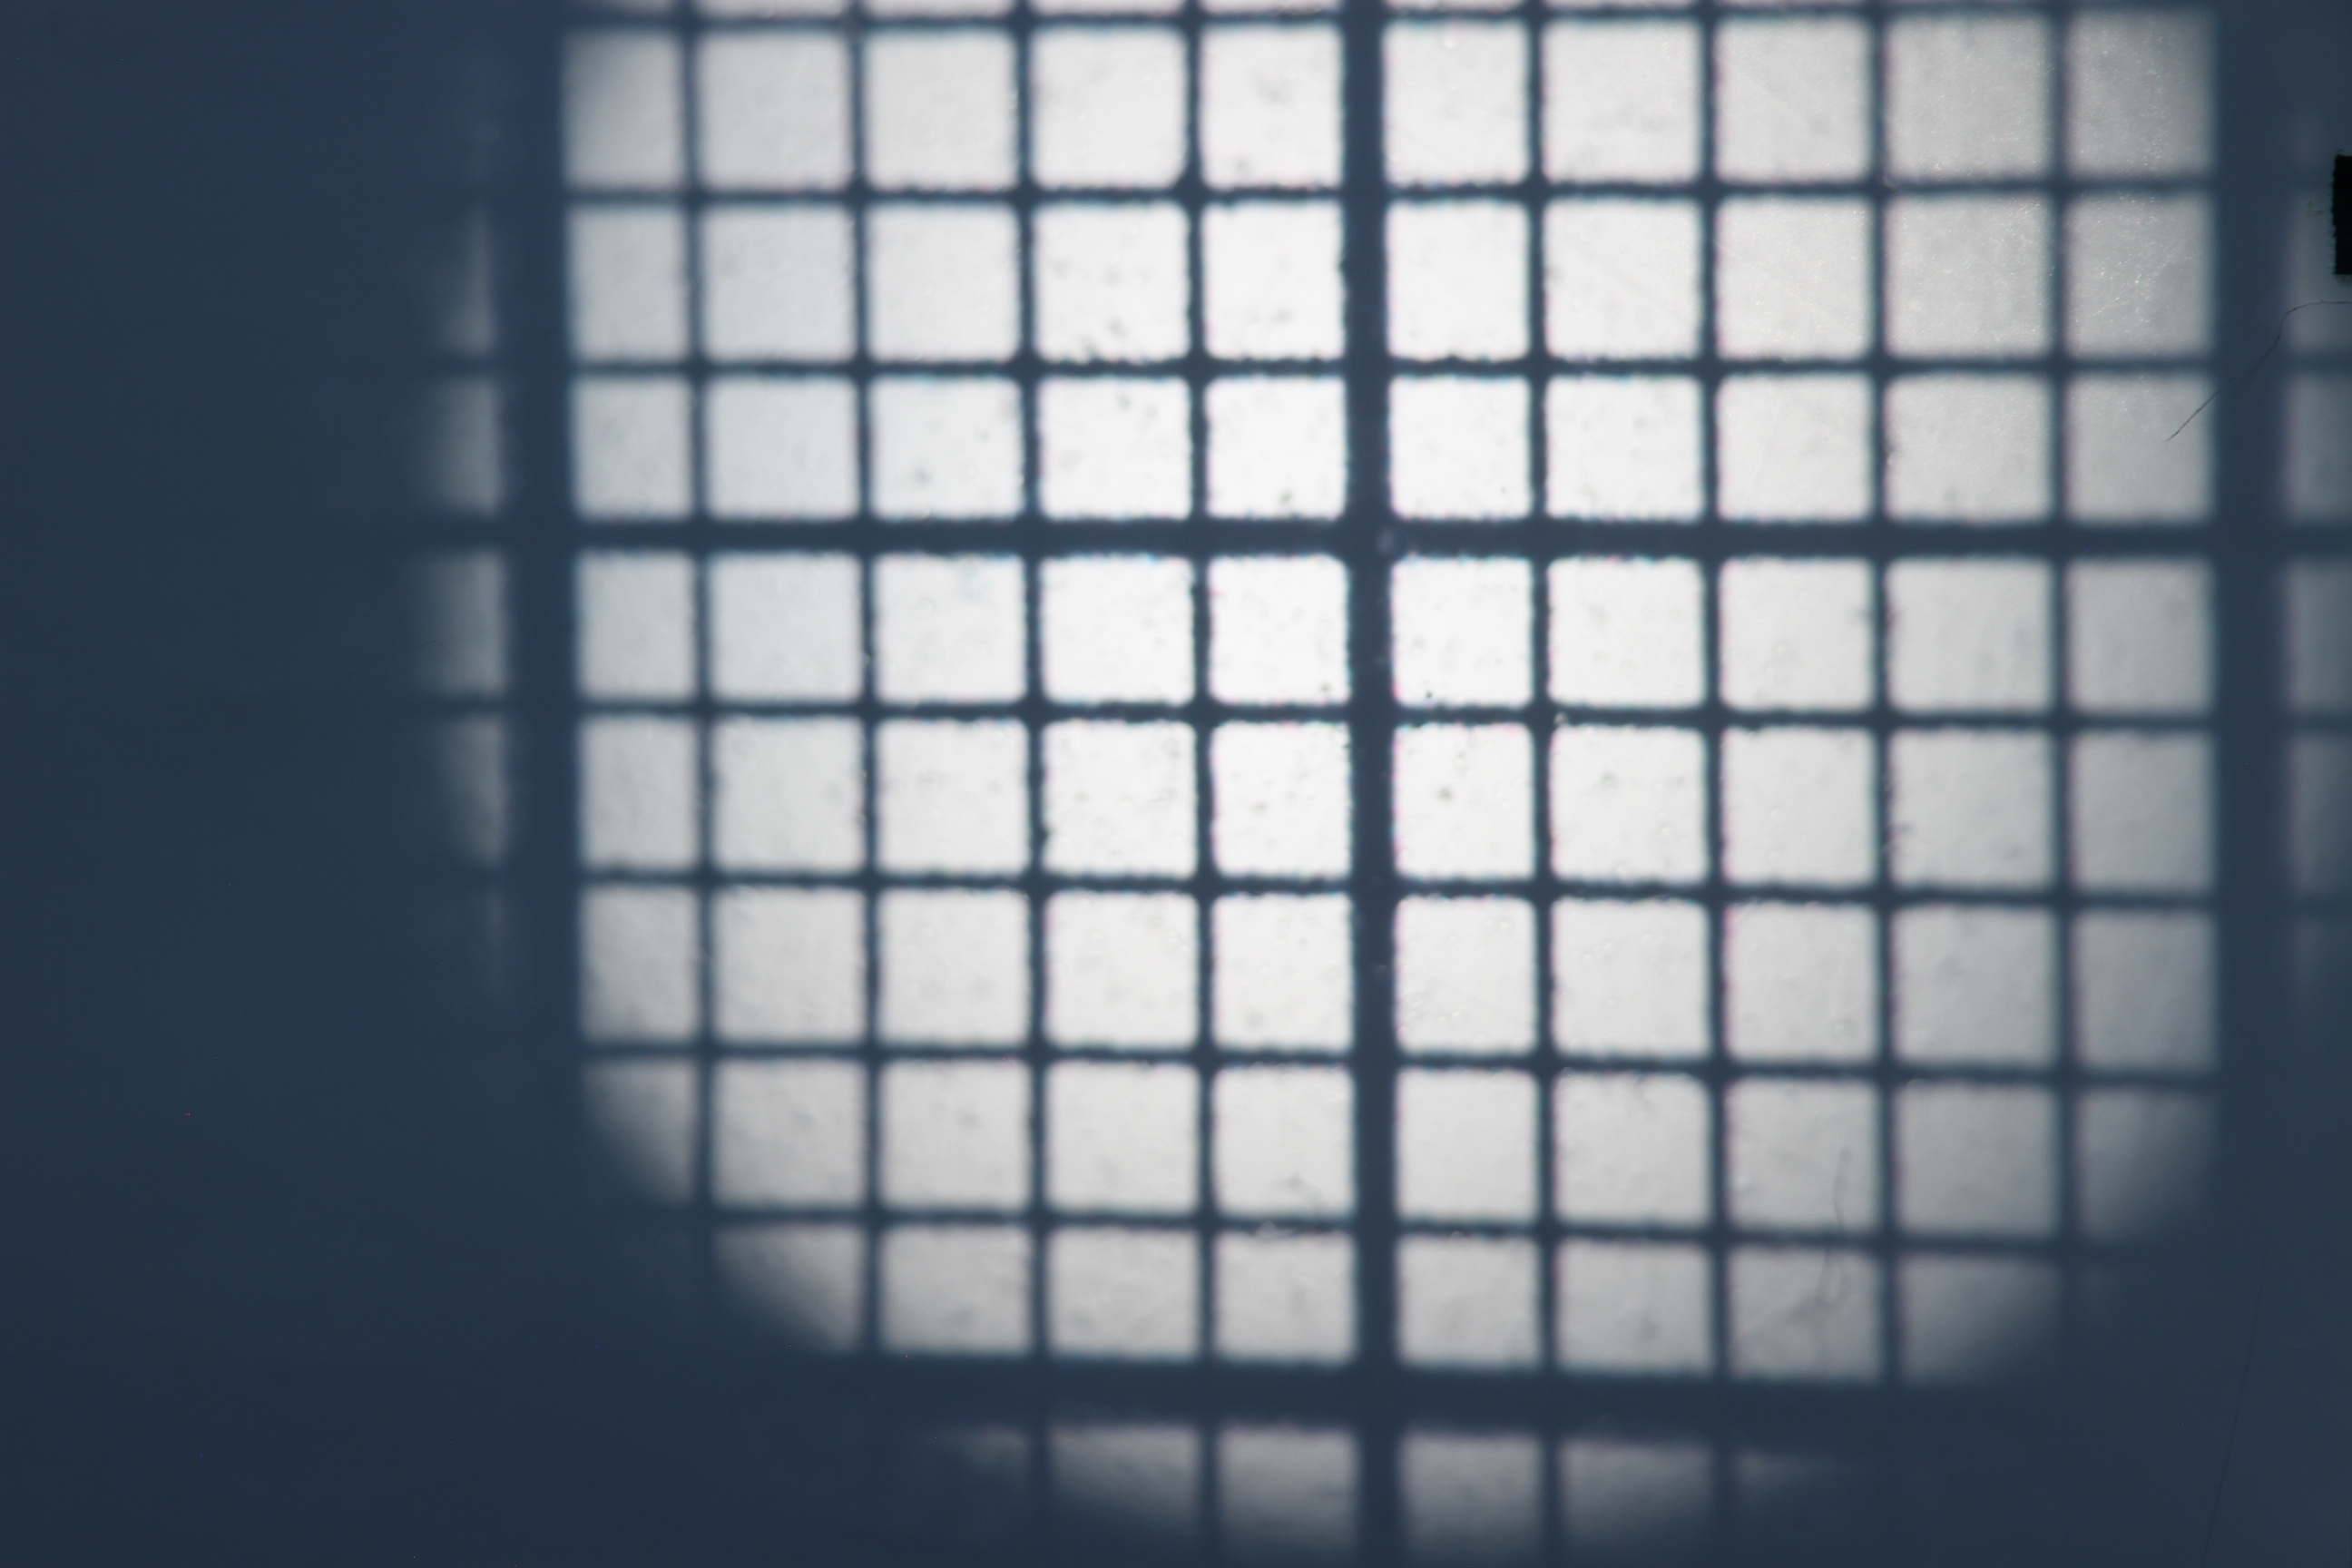
\includegraphics[width=\linewidth]{img/Verzeichnung/Prakt_Linsenfehler_2015_06_04_083}
		\label{fig:verzeichnung_korrigiert}
		\caption{Korrektur der Verzeichnung}
	\end{minipage}
\end{figure}

\subsection{chromatische Aberration}